\chapter{Results}

\begin{center}
    \textit{This chapter presents the outcomes of the project, including the functionality and performance of the developed application. It highlights the achieved results in relation to the project goals and requirements.}
\end{center}

\section{Overview of Delivered Product}
The application is an open-source, local, camera-based system designed to digitize \gls{otb} chess games in real time. It detects piece movements on a physical chessboard using image recognition and converts them into a \gls{pgn} file for digital viewing and analysis. The system runs entirely on common hardware,  such as a camera connected to a local machine running either Windows or Ubuntu, without relying on licensed software or cloud services. \\

The project is developed using open and freely available technologies. It follows  coding standards and best practices, ensuring the code is easy to understand, maintain, and extend. Comprehensive documentation supports future enhancements such as adding new chess variants, integrating additional hardware, or improving recognition models. The source code is published in a public Git repository with no restrictions on reuse or adaptation. \\

The delivered product is the final version of the application developed as part of this Bachelor’s thesis. It was created at the product owner's request, based on general requirements rather than detailed specifications. Design, architecture, and technology decisions were made by the development team and regularly reviewed with the product owner throughout the development process.

\section{Detection Performance Models}
\label{chesscam-metrics}
As a baseline for evaluating detection performance, results from the ChessCam repository were first considered \cite{github:chesscam}. These metrics represented the upper-bound performance of the models under ideal conditions. \\

Figure~\ref{fig:chesscam-piece-metrics} illustrates the performance of the piece detection model, which consistently shows high precision and recall throughout training. Both metrics quickly converged above 0.95, indicating stable and reliable detection performance \cite{wandb:piece-detection}. In contrast, Figure~\ref{fig:chesscam-xcorners-metrics} shows the results for xcorners detection, which demonstrated moderately lower performance. Precision and recall steadily improved over time and stabilized at approximately 0.8 and 0.75, respectively \cite{wandb:xcorner-detection}.

\begin{figure}[H]
\centering
\includegraphics[width=0.75\textwidth]{figures/results/machine-learning/piece-metrics.png}
\caption[Performance piece detection (ChessCam)]{Performance metrics for piece detection from the ChessCam repository \cite{wandb:piece-detection}.}
\label{fig:chesscam-piece-metrics}
\end{figure}

\begin{figure}[H]
\centering
\includegraphics[width=0.75\textwidth]{figures/results/machine-learning/xcorners-metrics.png}
\caption[Performance xcorners detection (ChessCam)]{Performance metrics for xcorners detection from the ChessCam repository \cite{wandb:xcorner-detection}.}
\label{fig:chesscam-xcorners-metrics}
\end{figure}

\section{API Testing Results}

All \gls{rest} and WebSocket endpoints were manually tested using Postman and a custom WebSocket simulator. Each endpoint returned the correct \gls{http} status codes and performed as expected. WebSocket connections remained stable, with all transmitted moves successfully received and rendered in the frontend interface. \\

No errors, dropped messages, or unexpected behaviors were observed during testing. These results indicate that the \gls{api} layer is functionally complete and enables reliable communication between the backend and frontend. As shown in Table~\ref{tab:api-test-results}, all \gls{api} endpoints passed testing and were deemed production-ready.

\begin{table}[h!]
\centering
\caption[API Test Summary]{Summary of test outcomes for \gls{rest} and WebSocket endpoints.}
\label{tab:api-test-results}
\begin{tabular}{L{0.3\linewidth}L{0.3\linewidth}L{0.3\linewidth}}
\toprule
\textbf{Endpoint} & \textbf{Test Performed} & \textbf{Result} \\
\midrule
\texttt{/reset/\{board\_id\}} & Reset board during simulation & \texttt{200 OK}, board reset confirmed \\
\texttt{/reset\_all} & Reset multiple boards & \texttt{200 OK}, all boards reset \\
\texttt{/boards} & Retrieve active board IDs & \texttt{200 OK}, correct IDs listed \\
\texttt{/video/\{id\}} & Stream board camera video & \texttt{200 OK}, stream rendered \\
\texttt{/moves/\{board\_id\}} & Receive move updates via WebSocket & Moves delivered and displayed in real time \\
\bottomrule
\end{tabular}
\end{table}


\section{Frontend}
\label{subsec:results-frontend}
The frontend of the application served as the user interface. It included a control panel for tournament organizers and a web application for spectators. The application was responsible for visualizing the chessboard and displaying ongoing moves. The frontend communicated with the backend via WebSocket to ensure real-time updates. \\

The control panel was a standalone administrative interface used by tournament organizers to configure and manage the tournament setup. It allowed the organizer to select the number of cameras, initiate the tournament, and reset boards between rounds, as shown in Figure~\ref{fig:control-panel}. This interface ensured centralized management of tournament operations. \\

\begin{figure}[h!] \centering \includegraphics[width=0.65\linewidth]{figures/results/frontend/control-panel/control-panel.png} \caption[Display of control panel]{The control panel used by the tournament organizers.}\label{fig:control-panel} \end{figure}

Once the organizer had configured the tournament through the control panel, the web interface became accessible to spectators. It allowed users to follow live games, switch views, and access system information across desktop and mobile devices via a responsive design. \\

The landing page was the tournament view, presenting an overview of all ongoing games. Each entry showed the board number, the players' names and ratings, and a link to follow the game live, as shown in Figure~\ref{fig:tournament-view-mocked}. \\



\begin{figure}[h!] \centering \fbox{\includegraphics[width=0.75\linewidth]{figures/results/frontend/tournament-view/mocked.png}}\caption[Display of tournament view]{A mocked demonstration of tournament view.}\label{fig:tournament-view-mocked} \end{figure}

The game preview page displayed miniature boards of all ongoing games, providing users with a quick overview and an easy way to select a game for detailed viewing, as shown in Figure~\ref{fig:game-preview}. It offered an efficient method to stay updated on multiple games simultaneously.

\begin{figure}[h!] \centering \fbox{\includegraphics[width=0.75\linewidth]{figures/results/frontend/game-preview/desktop.png}}\caption[Display of game preview]{A mocked demonstration of game preview.}\label{fig:game-preview} \end{figure}

One of the main pages in the web application was the board view, which presented a detailed display of a single game. It included a digital chessboard, move list, live camera feed, and evaluation bar, all updating in real time to create an engaging experience (Figure~\ref{fig:download-pgn}). Users could also download the current game's \gls{pgn} file via a dedicated button that saved it locally. \\

\begin{figure}[h!] 
    \centering 
    \fbox{\includegraphics[width=0.75\linewidth]{figures/results/frontend/download-pgn/download-pgn.png}}
    \caption[Display of board view]{A demonstration of downloading a \gls{pgn} file to a specific game.}
    \label{fig:download-pgn} 
\end{figure}

The downloaded file included a header containing key information such as the tournament name, date, and player names, followed by the recorded moves. It also indicated whether the game was still in progress. Upon completion, the result field displayed 1-0, 0-1, or $\frac{1}{2}$–$\frac{1}{2}$. Figure~\ref{fig:downloaded-pgn} shows an example of the file. \\

\begin{figure}[h!] 
    \centering 
    \fbox{\includegraphics[width=0.75\linewidth]{figures/results/frontend/download-pgn/downloaded-pgn.png}}
    \caption[PGN file and metadata]{The downloaded \gls{pgn} file to a specific game, opened in a code editor.}
    \label{fig:downloaded-pgn} 
\end{figure}

\section{Project Management}
\label{sec:results-project-management}
Although the project was initially structured according to the \gls{scrum} framework, its practical execution became more \gls{scrum}-inspired due to the absence of a dedicated \gls{scrum} Master and certain deviations from the full methodology. Each sprint began with a planning session in which tasks were selected from the product backlog based on priority and available team capacity. Sprint reviews were conducted at the end of each sprint to assess completed work and record outcomes. In addition, sprint retrospectives were held and documented, including reflections on workload distribution, communication challenges, and opportunities for process improvement. \\

Meeting routines were adapted according to team availability and project needs. Internal meetings were held as needed rather than on a fixed schedule, with most collaboration taking place informally during shared office hours. Nevertheless, short stand-up meetings were prioritized on a daily basis to maintain effective communication and ensure alignment. Biweekly meetings with the supervisor were consistently maintained, functioning as checkpoints for academic progress and clarification of requirements. Meetings with the product owner were arranged approximately once or twice per month and typically focused on feature validation, feedback, and adjustments. \\

GitHub was used consistently throughout the project for both task management and version control. Issues were linked to corresponding branches and categorized by type for example feature, enhancement, documentation. All code changes were submitted via pull requests, and no changes were pushed directly to the main branch. Peer review was strictly enforced as part of the workflow, with every pull request reviewed by at least one team member before merging. \\

Tasks were assigned to individual team members and tracked using GitHub Issues. Issues were labeled and moved through the workflow stages: \textit{No Status}, \textit{To Do}, \textit{In Progress}, and \textit{Done}. This workflow was followed consistently for larger development tasks. However, some minor items, particularly quick fixes and small adjustments, were occasionally completed outside of the issue board during periods of intensive development, resulting in slightly reduced traceability for those changes.\\

In addition to manual code review, automated workflows were implemented using GitHub Actions to support continuous integration and reduce human error. One workflow was configured to run Python unit tests on every push, ensuring code stability throughout development. Another workflow was responsible for automatically updating LaTeX-based documentation by cloning the relevant repository and pushing changes after each update, as shown in Figure~\ref{fig:workflow-latex}. These pipelines contributed to improved reliability, automation of repetitive tasks, and early detection of errors during development. \\

\begin{figure}[h!] \centering 
\includegraphics[width=0.75\linewidth]{figures/results/workflows/latex.png}\caption[Upload LaTeX workflow]{The workflow for update documentation with code.}\label{fig:workflow-latex} \end{figure}

\newpage

\section{Technical Achievements}

\subsection{Architecture Overview}
\label{subsec:diagrams}

To provide a comprehensive understanding of the system architecture and interaction flow, several \gls{uml} diagrams were created. These diagrams model different aspects of the live chess game digitization system, from component interactions and activity flow to user roles and use cases.

\subsubsection*{Use-Case Diagram}
\label{subsubsec:use-case-diagram}

The use-case diagram, shown in Figure \ref{fig:use-case}, identifies the system’s main actors and the primary functionalities they interact with. Admins are responsible for hardware setup and initiating the game recording process. Users, on the otherhand, access the game remotely to spectate. This diagram provides an overview of who interacts with the system and what capabilities are exposed, forming the basis for understanding system requirements and user expectations.

\begin{figure}[h!]
    \centering
    \includegraphics[width=0.75\linewidth]{figures/results/uml/use-case.png}
    \caption[Use-case diagram]{Use-case diagram outlining the system’s main actors and their interactions with key functionalities.}
    \label{fig:use-case}
\end{figure}  

\subsubsection*{Sequence Diagram}
\label{subsubsec:sequence-diagram}

The sequence diagram, shown in Figure \ref{fig:sequence}, illustrates the chronological flow of interactions between the system components and external actors. It begins with the admin initiating the game recording by setting up the camera, which captures and streams the board state to a local processing unit. The diagram emphasizes the communication between hardware (camera and local machine) and the \gls{ui}.


\begin{figure}[h!]
    \centering
    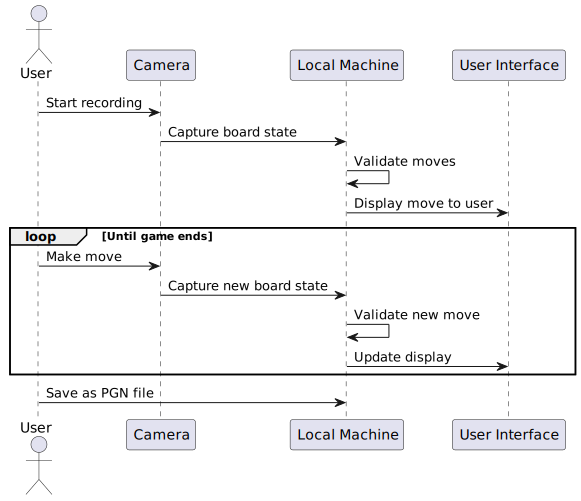
\includegraphics[width=0.75\linewidth]{figures/results/uml/sequence.png}
    \caption[Sequence diagram]{Sequence diagram showing the interaction flow between system components.}
    \label{fig:sequence}
\end{figure}

\newpage

\subsubsection*{Class Diagram}

The class diagram in Figure \ref{fig:class} provides a high-level overview of the system’s object-oriented design, detailing the core components involved in the chess digitization process. The central class, \texttt{App}, acts as the main entry point for the application, orchestrating the initialization of system services and user interface components. It interacts with the \texttt{BoardFactory} to generate multiple \texttt{Board} instances, each representing a physical chessboard, and connects to \gls{gui} elements such as \texttt{ProgressBarTopLevel} and \texttt{BoardResetSelectorTopLevel}, which support board resets and progress tracking. \\

Each \texttt{Board} object aggregates a \texttt{Camera} for video input and a \texttt{Detector} for move recognition using computer vision. It maintains a history of moves, manages WebSocket clients, and offers methods for validating and resetting board states. The \texttt{BoardService} class handles the overall control flow, managing boards, processing moves, and starting detector threads. Error handling is supported through a custom \texttt{CameraDoesNotExistError} exception. This structure ensures a separation of concerns, supporting modular development and maintainability across the data, control, and interface layers of the system.

\begin{figure}[h!]
\centering
\includegraphics[width=0.75\linewidth]{figures/results//uml/class.png}
\caption[Class Diagram]{Class diagram of the chess digitization system.}
\label{fig:class}
\end{figure}

\newpage

\subsubsection*{Package Diagram}

Figure \ref{fig:package-backend} illustrates the package structure of the backend system, organized around a modular architecture. The core logic resides in the \texttt{logic} package, which encapsulates domain-specific functionality such as board state detection, computer vision, mathematical operations, and supporting utilities. This modular breakdown, particularly in subpackages like \texttt{machine\_learning}, promotes separation of concerns and enhances reusability and testability. Alongside it, the \texttt{api} package handles external communication through submodules for data entities, service logic, and route definitions using FastAPI. Supporting components include static \texttt{resources} and the application entry point \texttt{main.py}, which binds the service and routing layers. This structure enables clean integration between backend services, data flow, and \gls{api} endpoints. \\

\begin{figure}[h!]
    \centering
    \includegraphics[width=\linewidth]{figures/results/uml/package-backend.png}
    \caption[Package Diagram for Backend]{Package diagram for the backend package structure.}
    \label{fig:package-backend}
\end{figure}

\newpage

On the frontend, shown in Figure \ref{fig:package-frontend}, the React application follows a conventional structure under the \texttt{src} directory. Key folders include \texttt{components} for reusable \gls{ui} elements like camera and board displays, \texttt{pages} for route-linked views, and \texttt{layouts} for defining common structural components across pages, such as headers or navigation bars. The \texttt{data} directory supports configuration or mock content during development. Outside \texttt{src}, the \texttt{public} folder holds static assets like \texttt{index.html}, while \texttt{App.tsx} and \texttt{index.css} define the main logic and styling. This organization supports maintainability and scalability by separating visual components, logic, routing, and configuration.

\begin{figure}[h!]
    \centering
    \includegraphics[width=\linewidth]{figures/results/uml/package-frontend.png}
    \caption[Package Diagram for Frontend]{Package diagram for the frontend package structure.}
    \label{fig:package-frontend}
\end{figure}

\newpage

\begin{figure}[H]
    \subsubsection*{Activity Diagram}
    \label{subsubsec:activity-diagram}
    
    \centering
    \begin{minipage}[t]{0.5\textwidth}
        \vspace{0pt}
        The activity diagram, shown in Figure \ref{fig:activity}, provides a high-level overview of the operational workflow during a chess game session. It models the continuous loop of capturing board states, detecting and validating moves, and updating the game state until the game ends. If a move is invalid, the system flags it but does not terminate the session. Once the game concludes, it is converted into a standard \gls{pgn} format. This diagram emphasizes the logical flow and decision-making process, reflecting the system’s role in automating and maintaining the integrity of live digitization.
    \end{minipage}
    \hfill
    \begin{minipage}[t]{0.45\textwidth}
        \vspace{0pt}
        \includegraphics[width=\linewidth]{figures/results/uml/activity-2.png}
        \caption[Activity Diagram]{Activity diagram illustrating the system workflow.}
        \label{fig:activity}
    \end{minipage}
\end{figure}



\begin{figure}[H]
    \subsubsection*{State Machine Diagram}
    \label{subsubsec:state-machine-diagram}

    \centering
    \begin{minipage}[t]{0.5\textwidth}
        Figure \ref{fig:state-machine} illustrates the state machine governing move detection and validation in the chess digitization system. The process begins in a waiting state, idling until a physical move is made. It then enters the detection phase, where the system captures and analyzes images using a machine learning model to identify the move. \\

        Once detected, the system transitions to a validation phase, where the move is checked for legality. Valid moves are displayed on the \gls{ui} and the system returns to its waiting state. Invalid moves lead to process termination. This diagram emphasizes the reactive, event-driven flow of the system, moving from detection to validation and feedback in response to user actions.
    \end{minipage}
    \hfill
    \begin{minipage}[t]{0.45\textwidth}
        \vspace{0pt}
        \includegraphics[width=\linewidth]{figures/results/uml/state-machine.png}
        \caption[State Machine Diagram]{State machine for move detection and validation.}
        \label{fig:state-machine}
    \end{minipage}
\end{figure}



\section{Testing and Quality Assurance}

\subsection{Machine Learning Model}
\label{machine-learning-test}

As described in Section~\ref{subsec:model-testing}, the model was evaluated using 100 games. Table~\ref{tab:accuracy-total} presents the overall move detection accuracy, both in total and broken down by piece type and color. The model achieved an overall accuracy of 90.6\%, successfully detecting 936 out of 1033 moves. Pawns had the highest detection rates, with over 98\% accuracy for both colors. In contrast, the model struggled particularly with black rooks with only 23.8\% accuracy.

\begin{table}[htbp]
\centering
\caption[Move detection accuracy total]{Move detection accuracy total.}
\label{tab:accuracy-total}
\begin{tabular}{lccc}
\toprule
\textbf{Category} & \textbf{OTB Moves} & \textbf{Successful Moves} & \textbf{Accuracy (\%)} \\
\midrule
\textbf{White Pieces} & & & \\
\hspace{1em}Pawn  & 244 & 242 & 99.2\% \\
\hspace{1em}Knight & 128 & 117 & 91.4\% \\
\hspace{1em}Bishop & 74  & 54  & 73.0\% \\
\hspace{1em}Rook   & 29  & 25  & 86.2\% \\
\hspace{1em}Queen  & 42  & 40  & 95.2\% \\
\hspace{1em}King   & 16  & 8   & 50.0\% \\
\midrule
\textbf{Black Pieces} & & & \\
\hspace{1em}Pawn  & 247 & 243 & 98.4\% \\
\hspace{1em}Knight & 78  & 75  & 96.2\% \\
\hspace{1em}Bishop & 65  & 47  & 72.3\% \\
\hspace{1em}Rook   & 21  & 5   & 23.8\% \\
\hspace{1em}Queen  & 84  & 76  & 90.5\% \\
\hspace{1em}King   & 5   & 4   & 80.0\% \\
\midrule
\textbf{Total} & 1033 & 936 & 90.6\% \\
\bottomrule
\end{tabular}
\end{table}


Table \ref{tab:board-type-accuracy} compares the success rates between the two physical board types used during testing. The wooden board performed slightly better than the plastic board, with a 91.2\% success rate compared to 89.9\%. This marginal difference may indicate a slightly more stable detection environment on the wooden surface. \\


\begin{table}[htbp]
\centering
\caption[Move detection accuracy board type]{Summary of total moves and success rate by board type.}
\label{tab:board-type-accuracy}
\begin{tabular}{lccc}
\toprule
\textbf{Board Type} & \textbf{Total Moves} & \textbf{Total Successful Moves} & \textbf{Success Rate (\%)} \\
\midrule
Plastic & 475 & 427 & 89.9\% \\
Wooden  & 558 & 509 & 91.2\% \\
\bottomrule
\end{tabular}
\end{table}


Figure \ref{fig:move-failures} shows the number of failed games (i.e., games where detection failed) grouped by the move number at which failure occurred. Bars are color-coded by board type. The majority of failures occurred within the first five moves, particularly at moves 2, 4, and 5. This trend suggests that the early game presents the greatest challenge for detection, potentially due to rapid development or ambiguity in piece positions. Notably, failures after move 9 were rare. \\


\begin{figure}[h!]
\centering
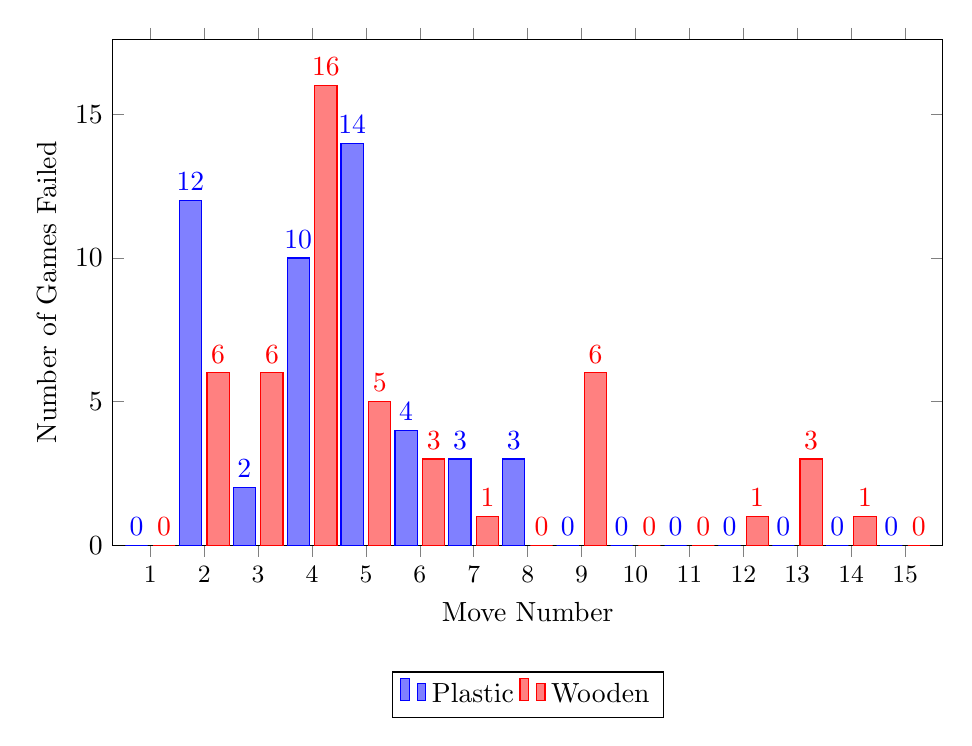
\begin{tikzpicture}
\begin{axis}[
    ybar,
    bar width=8pt,
    width=\textwidth,
    height=8cm,
    enlarge x limits=0.05,
    ymin=0,
    ylabel={Number of Games Failed},
    xlabel={Move Number},
    xtick={1,...,15},
    xticklabels={1,2,3,4,5,6,7,8,9,10,11,12,13,14,15},
    x tick label style={rotate=0, anchor=north, font=\small},
    legend style={at={(0.5,-0.25)}, anchor=north, legend columns=-1},
    nodes near coords,
    symbolic x coords={1,2,3,4,5,6,7,8,9,10,11,12,13,14,15},
    xticklabel style={font=\small},
]
\addplot+[style={fill=blue!50}] coordinates {
    (1,0) (2,12) (3,2) (4,10) (5,14) (6,4) (7,3) (8,3) (9,0)
    (10,0) (11,0) (12,0) (13,0) (14,0) (15,0)
};
\addplot+[style={fill=red!50}] coordinates {
    (1,0) (2,6) (3,6) (4,16) (5,5) (6,3) (7,1) (8,0) (9,6)
    (10,0) (11,0) (12,1) (13,3) (14,1) (15,0)
};
\legend{Plastic, Wooden}
\end{axis}
\end{tikzpicture}
\caption[Detection failures per move number]{Number of failed games per move number across plastic and wooden boards.}
\label{fig:move-failures}
\end{figure}


Table \ref{tab:different-errors} categorizes the types of detection failures for each board type. The majority of failures were due to a complete lack of detection within the allotted time window. Incorrect detections were less frequent but more common on the wooden board, accounting for 8 out of 48 failures, compared to just 1 on the plastic board. For a detailed breakdown of the chess games, including the sequences of moves, failure points, and detection statistics for each board type, see Appendix \ref{app:move-data-testing}.  \\

\begin{table}[htbp]
\centering
\caption[Different detection errors]{Frequencies of Different Detection Errors.}
\label{tab:different-errors}
\begin{tabular}{lccc}
\toprule
\textbf{Board Type} & \textbf{No Detection} & \textbf{Incorrect Detection} & \textbf{Total Failures} \\
\midrule
Plastic & 47 & 1 & 48 \\
Wooden & 40 & 8 & 48 \\
\midrule
\textbf{Total} & 87 & 9 & 96 \\
\bottomrule
\end{tabular}
\end{table}

\subsection{Wireframe}
\label{subsec:wireframe-results}

A total of eight individuals participated in the wireframe usability test, excluding project developers and stakeholders. While the sample size was limited, participants were intentionally selected to represent a broad range of ages, technical backgrounds, and familiarity with chess. \\

Overall, the feedback was generally positive. Participants were asked to rate their satisfaction on a 1–5 Likert scale. Figure \ref{fig:wireframe-test-results} shows the distribution of the ratings. The average scores from the feedback form were as follows:

\begin{itemize}
    \item The \textbf{overall user experience} received an average rating of \textbf{4.63} out of 5.
    \item The \textbf{tournament view page} received the highest average rating of \textbf{4.75}.
    \item The \textbf{board view page} received a slightly lower average rating of \textbf{4.38}.
\end{itemize}

Participants commented that the interface was easy to navigate and that the layout felt intuitive. The tournament view, in particular, was praised for its clarity and structure. Several testers without prior experience using chess-related software indicated that the interface felt approachable and visually clear. \\

However, participants also suggested a few areas for improvement:

\begin{itemize}
    \item Adding a full-screen function for the video feed.
    \item Enhancing the visual design of some \gls{ui} elements for improved aesthetics.
    \item Supporting multiple languages for users who do not speak English.
\end{itemize}

While these findings are based on a small participant group, they offer early indications that the interface is both accessible and functional for a wide range of users. These insights will guide further development and refinement of the user interface.

\begin{figure}[h!]
\centering
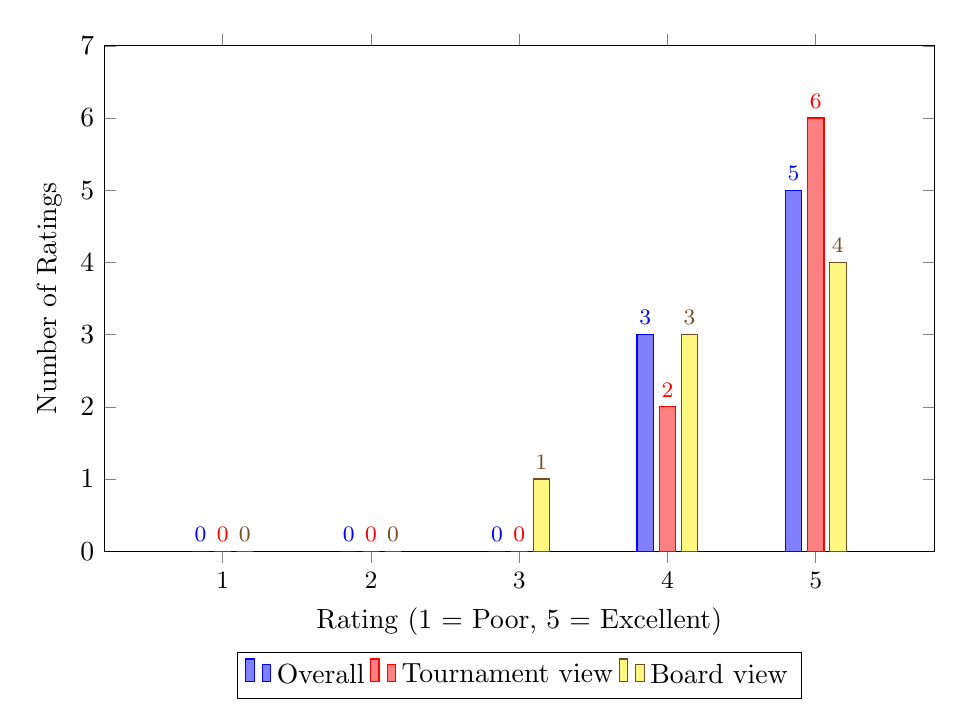
\begin{tikzpicture}
\begin{axis}[
    ybar,
    bar width=6pt,
    width=\textwidth,
    height=8cm,
    enlarge x limits=0.2,
    ymin=0,
    ymax=7,
    ylabel={Number of Ratings},
    xlabel={Rating (1 = Poor, 5 = Excellent)},
    symbolic x coords={1,2,3,4,5},
    xtick=data,
    x tick label style={rotate=0, anchor=north, font=\small},
    legend style={
        at={(0.5,-0.2)},
        anchor=north,
        legend columns=3
    },
    nodes near coords,
    nodes near coords style={font=\footnotesize},
    every node near coord/.append style={
        /pgf/number format/.cd,
        fixed,
        precision=0,
        /tikz/ifthenelse/.code={
            \ifnum\pgfplotspointmeta=0
                \pgfkeys{/pgfplots/disable node}
            \fi
        }
    }
]
\addplot+[style={fill=blue!50}] coordinates {
    (1,0) (2,0) (3,0) (4,3) (5,5)
};
\addplot+[style={fill=red!50}] coordinates {
    (1,0) (2,0) (3,0) (4,2) (5,6)
};
\addplot+[style={fill=yellow!50}] coordinates {
    (1,0) (2,0) (3,1) (4,3) (5,4)
};
\legend{Overall, Tournament view, Board view}
\end{axis}
\end{tikzpicture}
\caption[Satisfaction rating distribution]{Distribution of satisfaction ratings from participants across different interface views.}
\label{fig:wireframe-test-results}
\end{figure}



\subsection{Color Palette}
\label{subsec:results-color-palette}
Voting revealed a mix of preferences: some participants favored the light mode from palette \#08 and the dark mode from palette \#07, while others selected the board design from palette \#05 or the move-highlighting style from palette \#14. \\

Rather than selecting a single predefined palette, the final color scheme was assembled by combining the most highly rated elements across the top-voted variations, yielding a more tailored, user-informed visual design. Figure \ref{fig:color-palette-results} shows the distribution of votes across all tested palettes; the full set of prototypes appears in Appendix \ref{app:color-palettes}.

\begin{figure}[h!]
\centering
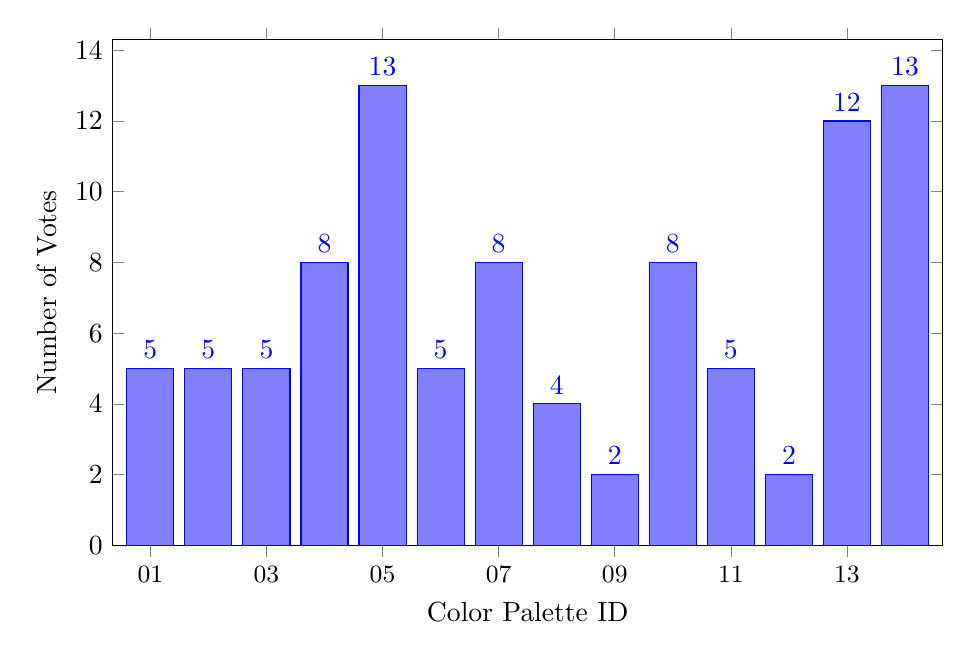
\begin{tikzpicture}
\begin{axis}[
    ybar,
    bar width=17pt,
    width=\textwidth,
    height=8cm,
    enlarge x limits=0.05,
    ymin=0,
    ylabel={Number of Votes},
    xlabel={Color Palette ID},
    xticklabels={01,02,03,04,05,06,07,08,09,10,11,12,13,14},
    x tick label style={rotate=0, anchor=north, font=\small},
    nodes near coords,
    symbolic x coords={01,02,03,04,05,06,07,08,09,10,11,12,13,14},
    xticklabel style={font=\small},
]
\addplot+[style={fill=blue!50}] coordinates {
    (01, 5) (02, 5) (03, 5) (04, 8) (05, 13) (06, 5) (07, 8) (08, 4) (09, 2) (10, 8) (11, 5) (12, 2) (13, 12) (14, 13)
};
\end{axis}
\end{tikzpicture}
\caption[Votes per color palette]{Distribution of Votes Across Different Color Palettes.}
\label{fig:color-palette-results}
\end{figure}